\chapter{绪论}
\label{cha:chap1}
\section{研究背景和研究意义}
\label{sec:1.1}
\subsection{研究背景}
\label{sec:1.1.1}
人类通过双眼来探索与发现世界,在接收外部信息的方式中,有不到三成来自于听觉、触觉、嗅觉等感受器官,而超过七成、最丰富、最复杂
的信息则通过视觉进行感知的。计算机视觉便是一种探索给计算机装备眼睛(摄像头)与大脑(算法)的技术,以使计算机能够自主独立的控
制行为、解决问题,同时感知、理解、分析外部环境。

20世纪60年代,计算机视觉得到了最初的发展,该阶段的研究重心主要体现在如何从二维图像中恢复出如立方体、圆柱体等立体化的三维形
状,解释各个物体的空间位置关系。1982年David Marr从信息处理的角度对数学、神经生理学、计算机图形学等学科的研究成果进行了归纳
总结,并在此基础上提出了一系列计算机视觉理论,经典Marr视觉信息处理过程如图~\ref{fig:introduction_Marr}所示。得益于这个完
整明确的理论体系,计算机视觉得到了蓬勃的发展,它的核心思想是从二维图像恢复三维结构。
\begin{figure}[H] % use float package if you want it here
  \centering
  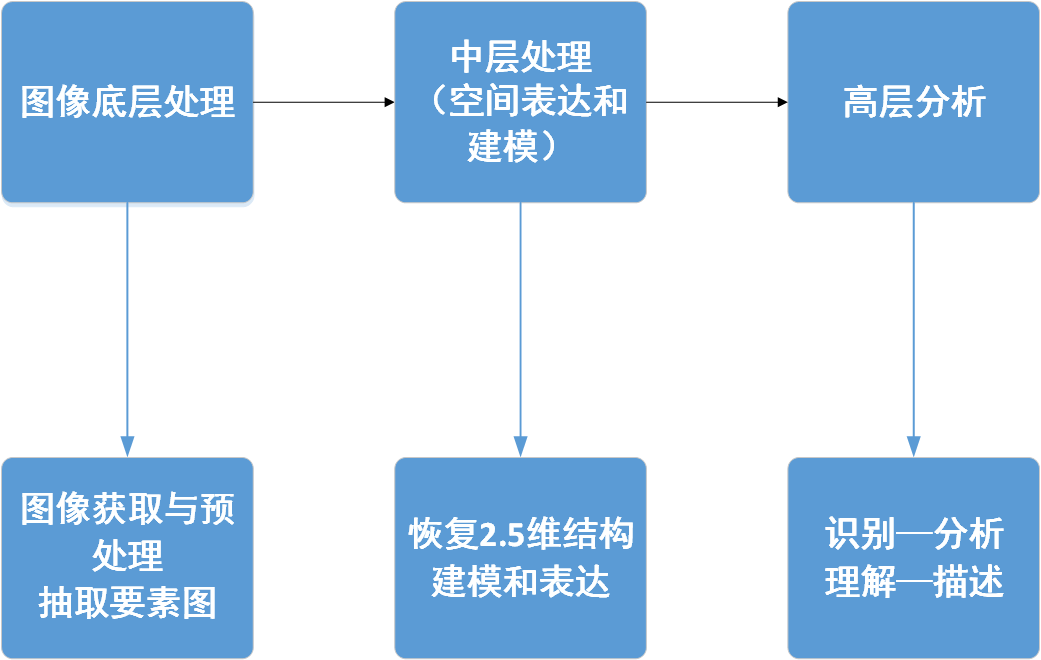
\includegraphics[height=6cm]{introduction_Marr.png}
  \caption{经典Marr视觉信息处理过程示意图}
  \label{fig:introduction_Marr}
\end{figure}
近年来,图像的三维重建在计算机视觉中发挥了很大的作用,并且在质量和性能上有了较大的提升。其主要应用是自动地对于难以建模的对象
建模,加快了图像运用的建模过程。这种技术需要处理大量的数据,可以使用于室内和室外的场景, 而不受控制的环境通常影响室外场景,如
密集建筑群,或者复杂的原始森林等。对于这些场景,虚拟现实和计算机模拟可以被用来分析工作环境和工作难度等方面,三维图像重建技术
本身被视为一个生成3D模型的技术。快速有效完整重建类似于雕塑三维物体目标的三维模型成为目前的研究方向。由连续图像的三维重建主要
是指从二维图像序列中的获取物体的信息并进行三维重建。然而,这个领域并没有引起人们足够的重视,因此本文将对三维重建的具体原理以及
改善展开讨论。

当前在一些工业场景中,需要对其中场景进行测量,主要包括场景的高度,面积,体积,甚至于温度,湿度分布等,传统方式中主要采用雷
达扫描场景的方式来进行,但考虑到该雷达本身成本较高,受场景的限制也很大,在室外环境或者大尺度环境下,就难以发挥作用。现在更多
采用计算机视觉的方式来解决这些问题,可以根据三维重建的点云结果测量以上所描述的几何特性,这样做只需要结合摄像机和测量算法即
可实现,可以很简易的复现在多种场合中。
\subsection{研究意义}
\label{sec:1.1.2}
本文的研究目标是让无人机能够在全封闭或者半封闭的环境中,完全基于视觉的方法完成自主飞行任务,并且在飞行的过程中,采集待测物
体的实拍图像,进行三维重建,最终根据三维重建的点云结果测算待测物体的体积值。

传统无人机的飞行都需要依靠操作员手动控制,或者是基于GPS定位结果进行巡航,本文提出了一种完全基于纯视觉的方法来进行无人机定位
的导航得到的方法,该方法可以在全封闭无GPS的环境中,为无人机提供定位信息,解决了场景限制的问题,并且整个无人机的飞行过程可以
完全自动化的运行,并对场景进行图像采集。

从二维图像重建三维立体具有重要的研究价值和潜在经济社会价值,其核心技术是通过运动来恢复结构。三维重建系统在不同的应用领域有
着不同的预设条件和技术要求,主要包括医学领域的重建系统,机器人导航相关实时重建系统,工业领域包括3D打印在内的室内高精度重建
系统,以及摄影测量领域实景三维重建系统。 三维重建已能提供完整方案,但传统三维重建算法得到的点云结果存在精确度不高,场景无
法闭合等问题,本文提出一种结合SLAM结果的三维重建方法,拟生成一个高精度,强鲁棒的点云地图。

有关实景物体三维测量,传统方法常采用激光雷达,声波等方案,这些方案成本较高,且对场景有限制要求要求,本文提出了一种基于三维
重建后的点云结果进行体积估计的方法,可以极大降低成本且能够在多重场合下复用算法。

因此基于无人机自主飞行采集图像数据的三维重建和体积测量有着十分重要的工程意义,并且在很多场合下,整体流程可靠性和可行性都得
到充分验证。


\section{国内外研究现状}
\label{sec:1.2}
本文主要涉及到的理论方法有及时定位与地图构建(Simultaneous localization and mapping,简称SLAM),三维场景重建,
视觉体积测量等几个方面对国内外研究现状和发展动态进行描述。
\subsection{SLAM的研究现状}
\label{sec:1.2.1}
SLAM(即时建图与定位)是一种在定位导航的同时,进行构图的技术\cite{cadena2016past}。最早的SLAM技术还不是使用视觉的方法,
而是使用声波传感器或者激光以及惯性测量单元实现环境建模和自身定位,直到21世纪,Stephen Se等人首次使用图像的特征点实现视觉
SLAM\cite{se2002mobile},之后由$Davison$使用$EKF$框架实现了最早的单目实时SLAM系统\cite{davison2003real},奠定了单目系统
的基础;Davison在2007年成功实现基于单相机的纯视觉SLAM系统,算法的关键是在线建立2D点到3D点的映射关系,并且使用实时运动模
型估计相机的位置\cite{davison2007monoslam};Mur-Artal使用ORB特征点作为地图构建特征点,大幅度降低了点云的数量,并且使用
回环检测的方法使定位与建图的精度都大幅提升\cite{mur2015orb};随着硬件计算能力和数据储存的提升,提取目标深度信息的技术得
到了很大的发展,戚传江等人使用2D slam的解决方案,采用多传感器数据融合的方法,完成多自由度位姿检测,拓展了SLAM的应用场
景;Whelan的实验通过使用体积融合的方法实现了实时大范围的稠密RGB-D的SLAM系统\cite{whelan2015real}。

Durrant-Whyte和Bailey首先对前20年里SLAM的发展做出了详细的历史回顾,
并提出了概率方法和数据融合\cite{Gibbens2000A,durrant2006simultaneous},Aulinas等人提出在SLAM中添加滤波方法减少噪音影响
\cite{cadena2016past},Grisetti等人就SLAM后端进行详细阐述\cite{grisetti2010tutorial},Dissanayake研究了SLAM的基本性质,
包括可观测性、收敛性和一致性等\cite{dissanayake2011review}。近几年来,SLAM的发展更多的开始和机器人领域相结合, 
Saeedi提出了多协同机器人SLAM解决方案\cite{saeedi2016multiple},Stachniss发布了在SLAM领域机器人开发
手册\cite{stachniss2016simultaneous}。

应用到目标跟踪领域,单纯点云集还是无法满足要求,因此需要将点云数据语义化,Reiger使用关系树的方法实现物体的语义识别
\cite{sarkar2012slam},这项技术对于目标跟踪是很重要的;之后Sarkar在Reiger的研究基础上结合FastSLAM的方法,使得识别速度
更快,鲁棒性更强;Zhang, G等人使用基于线条的SLAM算法\cite{zhang2015building}提高物体识别的准确率,该方法能够对物体的边
沿与轮廓进行稳定的识别。

当使用单目相机运行SLAM算法时,依旧还存在很多的挑战,ORB-SLAM2\cite{mur2017orb}和LDSO\cite{gao2018ldso}
可能是目前单目SLAM中最先进的方法。然而,这些方法还存在很多的局限性,无地图复用,无法纯旋转,场景需丰富等,
并且用于重定位的方法\cite{galvez2012bags}在视点变化、重复模式和随时间变化时的性能有限。另一种估计相机姿态的方法是使用放置
在环境中的人工标记,最近的SPM-SLAM\cite{munoz2019spm}解决了之前描述的一些限制,它使用二维码而不是自然特征,但是也存在场
景中摆放大量二维码的问题。UcoSLAM\cite{munoz2019ucoslam}则提出了一种结合自然点和人造二维码的SLAM运行方法。

\subsection{三维重建的研究现状}
\label{sec:1.2.2}
照相机/摄像机是将一个三维场景或物体投影到二维平面上,但是在降维的过程不可避免地会损失存在信息,而利用三维重建技术,就是从获
取到的二维图像中复原原始三维场景或物体,三维重建的结果如图~\ref{fig:3d_constr}所示。

\begin{figure}[H] % use float package if you want it here
    \centering
    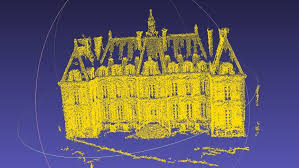
\includegraphics[height=8cm]{3d_constr.png}
    \caption{三维重建结果示意图}
    \label{fig:3d_constr}
  \end{figure}

三维重建技术就是获取环境中物体的三维信息,从而确定不同物体所在位置并建立相应的空间模型~\cite{feng2018reconstruction},具有高
效率的三维重建技术也已经被应用在众多领域当中,其中包括城镇建模、无人作战、文物保护和地图重建等,相关的重建算法及流程也愈加完善
~\cite{liu2018application}。基于图像的三维重建从获取多视图图像开始,逐步通过相应的算法恢复场景中物体的三维结构
\cite{rupnik20183d}。基于图像的三维重建技术是当今计算机视觉领域的热门方向~\cite{zhang2017data},
常见的三维重建的方法如表~\ref{tab:3Dconstruction}所示。


\begin{table}[h]
  \centering
  \caption{常见三维重建方法}
  \label{tab:3Dconstruction}
  \begin{tabular}{C{3.4cm}C{1.6cm}C{0.8cm}C{3.4cm}C{3.4cm}}
  \toprule
  \textbf{方法} & \textbf{复杂度} & \textbf{实时} & \textbf{效果}& \textbf{应用场景} \\
  \midrule
  明暗恢复形状法\cite{nayar1994shape}    & 简易   &否 & 光照影响大,效果较差 &难以用于室外           \\
  几何光学测量法\cite{choi1999three}    & 人工调节   &否 &效果精细 &难以用于贫纹理环境           \\
  投影光栅相位法\cite{srinivasan1984automated,颜国霖2010基于光栅相位法三维重构技术研究}    & 至少3幅图像   &否 & 弱光环境效果好 &难以用大尺度场景          \\
  单激光线扫描法\cite{黄俊春2009基于彩色结构光的实时三维重建}    & 设备复杂   &是 &效果精细,速度快 &适用于小尺度场景           \\
  彩色条纹结构光法\cite{izquierdo1999sub}    & 仅需要一张彩图   &是 &精度低,鲁棒性强 &适用于彩色场景           \\
  复合结构光测量法\cite{takeda1983fourier}    &仅需要一张完整图 &是 & 精度高 &适用于投影和实物距离远           \\
  双目视差法\cite{黄俊春2009基于彩色结构光的实时三维重建}    & 设备复杂且耗时   &是 &大尺度效果好&适用于大多数场景           \\
  \bottomrule
  \end{tabular}
\end{table}


基于单目视觉的三维重建技术是仅使用一台相机来进行三维重建的方法, 这种方法简单方便、灵活可靠、使用范围广, 可以在
多种条件下进行非接触、自动、在线的测量和检测,主要方法为运动恢复结构法(SfM),常用的SfM方法采用的是多视角几何法。
通常, 包括以下四个步骤: 

1)特征提取与匹配。特征提取是首先用局部不变特征进行特征点检测, 再用描述算子来提取特征点。Moravec~\cite{moravec1977techniques}
提出了用灰度方差来检测特征角点的方法。Harris~\cite{harris1988combined}在Moravec算法的基础上,提出了利用信号的基本特性来提取图像角点的H a r r i s 算法。
Smith等人~\cite{smith1997susan}提出了最小核值相似区,即SUSAN算法。Lowe~\cite{lowe2004distinctive}提出了一种具有尺度和旋转不变性的局部特征描述算子,
即尺度不变特征变换算子, 这是目前应用最为广泛的局部特征描述算子。Bay~\cite{bay2008speeded}提出了一种更快的加速鲁棒性算子。特征匹配是在两个输入视图之间寻找若干组最相
似的特征点来形成匹配。传统的特征匹配方法通常是基于邻域灰度的均方误差和零均值正规化互相关这两种方法 。
Grauman等人~\cite{grauman2007pyramid}提出了一种基于核方法的快速匹配算法,即金字塔匹配算法。Photo Tourism系统在两两视图间的局部匹配时采用了基于近似最近邻搜
索\cite{mount1998ann}的快速算法。

2)多视图几何约束关系计算。多视图几何约束关系计算就是通过对极几何将几何约束关系转换为基础矩阵的模型参数估计的过程。Longuet-Higgins~\cite{longuet1981computer}最早提出
多视图间的几何约束关系可以用本质矩阵在欧氏几何中表示。Luon~\cite{luong1992matrice}提出了解决两幅图像之间几何关系的基础矩阵。与此同时, 为了避免由光照和遮挡等因素造成
的误匹配, 学者们在鲁棒性模型参数估计方面做了大量的研究工作, 在目前已有的相关方法中, 最大似然估计法、最小中值算法、随机抽样一致性算法三种算法使用最为普遍。

3)优化估计结果。当得到了初始的射影重建结果之后, 为了均匀化误差和获得更精确的结果, 通常需要对初始结果进行非线性优化。在SfM中对误差应用最精确的非线性优化方法就是光束法平差。
光束法平差是在一定假设下认为检测到的图像特征中具有噪音, 并对结构和可视参数分别进行最优化的一种方法。近年来, 众多的光束法平差算法被提出, 这些算法主要是解决光束法平差有效
性和计算速度两个方面的问题。Ni~\cite{ni2007out}针对大规模场景重建, 运用图像分割来优化光束法平差算法。
Engels~\cite{engels2006bundle}针对不确定的噪声模型,提出局部光束法平差算法。Lourakis~\cite{lourakis2009sba}提出了可以应用于超大规模三维重建的稀疏光束法平差算法。

4)得到场景的稠密描述。经过上述步骤后会生成一个稀疏的三维结构模型, 但这种稀疏的三维结构模型不具有可视化效果, 因此要对其进行表面稠密估计, 恢复稠密的三维点云结构模型。
近年来, 学者们提出了各种稠密匹配的算法。Lhuillier等人~\cite{lhuillier2005quasi}提出了能保持高计算效率的准稠密方法。Furukawa~\cite{furukawa2009accurate}提出的基于
面片的多视图立体视觉算法是目前提出的准稠密匹配算法里效果最好的算法。

\subsection{基于视觉体积测算的研究现状}
\label{sec:1.2.3}
在测量领域,测量精度、测量速度、测量数字化和自动化程度要求不断提高,传统的接触式测量已经无法满足需要,基于纯视觉的非接触式测量方法具有结构简单、测量精度高、实时性好可复
用等特点以满足测量要求~\cite{chang2011parkinson}。目前,国内外很多的科研机构对光斑定位、CCD 自动聚焦调整、测量误差等不足问题进行了研究,并提出了相应的优化方法
~\cite{chang2011parkinson}。在实际应用领域,如德国OPTO NCDT 系列和日本 LK 系列、LC 系列等激光三角测量传感器在测量精度、速度等性能方面也比以前有较好的提高~\cite{cigada2010laser}。

物料体积的测量是工矿企业、港口码头等领域进行库存盘点和物料管理重要的工作,其中堆积物体是典型的物料体积测量,如钢铁冶金企业和矿石企业对物料体积的测量
\cite{wang2013research} 、港口码头对集装箱及堆积货物量\cite{chang2010bulk}或船体\cite{yuntao2014bias}的测量、甚至集装箱或船舱内货体积的测量~\cite{shi2014study} ,
都为合理利用资源和安排生产,提高生产效率发挥了重要作用。根据测量原理的不同,物料体积测量技术主要分为激光传感测量~\cite{ren2013research} 和计算机视觉测量
~\cite{dong2015study,liu2009distance},其中激光测量具有非接触、长距离和抗干扰的优点~\cite{rosen2012variation,meili2015design,shi2013study},更适合在户外大范围
测量的应用。在视觉测量方面,主要是在获取被测物体的点云之后采用剖分法~\cite{Guo2014Resolution,zhang2010remote}、凸包~\cite{bi2013canopy} 、切片法~\cite{shi2014study}
等方法进行体积计算。 

对于室内场景大型堆体的测量工作,熊友辉~\cite{熊友辉2003便携式激光盘煤系统原理及应用} 提出一种便携式激光测量仪,通过多站人工打点的方式进行盘点,虽然该仪器存在测量周期长、
精度差、人为影响大等缺点,但仍是现在堆场测量的常用方法。张德津等~\cite{张德津2012基于多传感器集成的堆场激光测量技术应用}提出了一种基于多传感器的固定式激光测量方法,该方
法将激光扫描仪安装在外界载体(如取料机等)上对堆场进行测量。盛业华等~\cite{盛业华2010地面三维激光扫描点云的多站数据无缝拼接} 提出了一种基于三维激光扫描点云的多站拼接方
法,该方法围绕被测目标布设多个测量点,将各测量获得的点云进行拼接进而获得完整的被测堆体模型。张小虎等~\cite{张小虎2011投影轮廓线辅助下的堆场三维形貌摄影测量研究}提出了激
光投影线辅助下的堆场三维形貌摄影测量方法,该方法围绕被测目标布设多个测量点,将各测量获得的点云进行拼接进而获得完整的被测堆体模型。王海波等~\cite{王海波2013大型露天料场激光测量方法研究}
提出了车载式多站盘点系统。


\section{待解决问题}
\label{sec:1.3}
当前基于无人机自主飞行采集图像数据进行三维重建以及体积测量的方案还存在很多的待解决问题,如:\\
(1)	无人机在完全封闭环境中依靠纯视觉进行定位和建图,难以获取高精度的飞行位姿和地图信息。\\
(2)	基于三维重建算法对场景进行三维重建时,面临整个流程耗时长,输出点云噪音点大,需要对传统三维重建进行提升,以获取高精度
强鲁棒性的大尺度地图。\\
(3)	基于三维点云的体积测算,点云中缺少水平面信息,尺度信息,导致无法直接获取到体积真值。
\section{主要研究内容和技术路线}
\label{sec:1.4}
本文将针对目前无人机在无GPS的密闭环境中进行自主飞行存在的问题,采用计算机视觉的方式建立一套稳定,高精度的无人机自主定位系
统,并对采集到的图像作为输入开发出一套能够生产高精度,强鲁棒的三维重建系统。针对获取到的三维点云,提出估计尺度,确定水平面
的方法以获取感兴趣区域的堆体体积本文将针对上述功能开发出一套完整、全自动化的系统。所研究系统将得到以下指标:\\
1)	建立一套无人机自动定位凶系统,使得无人机自主定位结果与真实GPS定位数值误差在0.5米以内,位置差距在2$\%$之内。\\
2)	建立一套基于视频流,并融合SLAM结果的和高精度三维重建系统,能够针对各种室内外的大尺度建筑物场景实现三维重建,场景场能将
误差控制在20cm以内。\\
3)	建立一套堆体体积自主测量系统,可以快速估计出点云的尺度,水平面方程与堆体体积,测量误差控制在2$\%$之内。\\
4)	建立一套基于无人机自主飞行采集图像数据进行三维重建以及体积测量的完整方案,实现快速全自动的测量流程。

结合研究内容,完成理论研究,系统实现以及测试实验与分析,技术路线如图~\ref{fig:introduction_pipeline}所示。
\begin{figure}[H] % use float package if you want it here
  \centering
  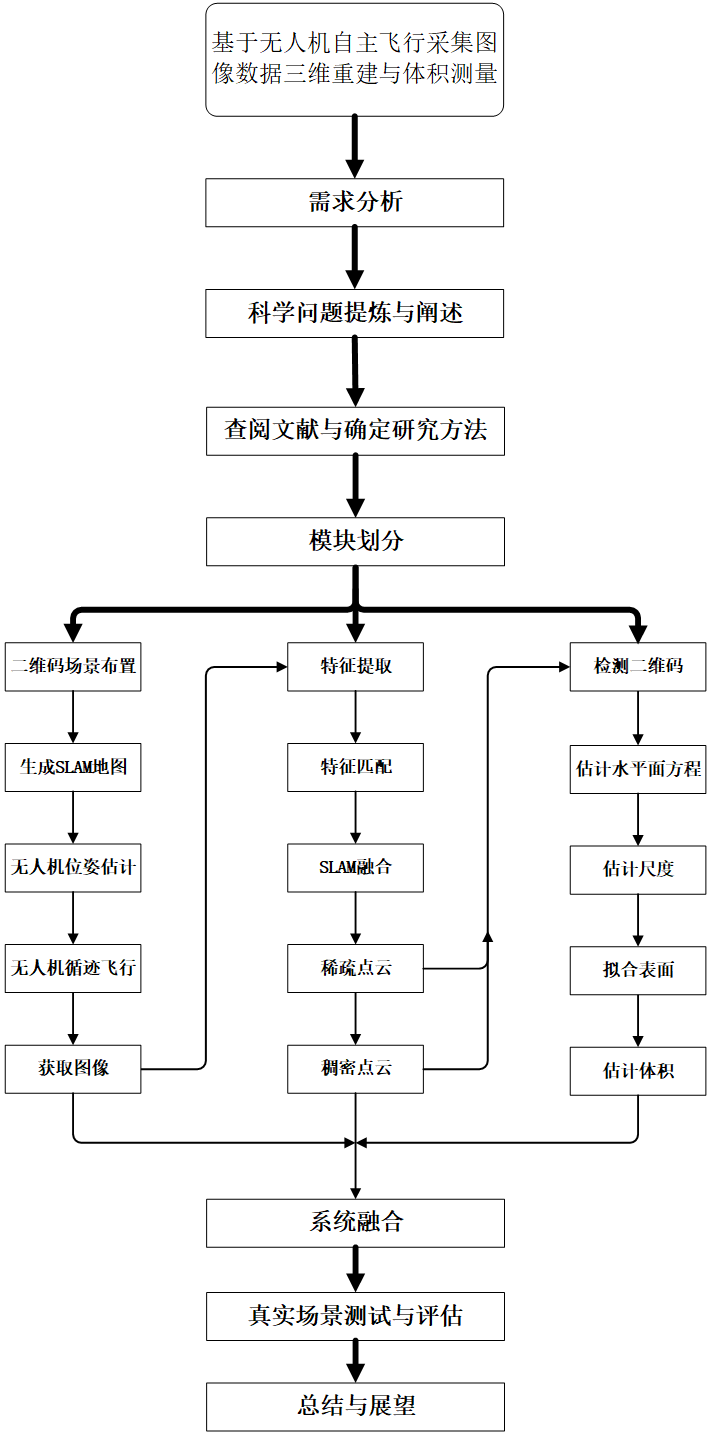
\includegraphics[height=22.5cm]{introduction_pipeline.png}
  \caption{技术路线图}
  \label{fig:introduction_pipeline}
\end{figure}
\section{章节安排}
\label{sec:1.5}

